\documentclass[12pt,oneside,letterpaper]{article}
\usepackage[margin=1in]{geometry}
\usepackage{listings}
\lstset{language=C++,
                basicstyle=\ttfamily,
                keywordstyle=\color{blue}\ttfamily,
                stringstyle=\color{red}\ttfamily,
                commentstyle=\color{green}\ttfamily,
                morecomment=[l][\color{magenta}]{\#}
}
\usepackage{color}
\usepackage{graphicx}
\usepackage{hyperref}
\usepackage{amsmath}
\usepackage{amsfonts}
\usepackage{amsthm}
\newtheorem{definition}{Definition}

\title{OpenGM Demo}
\author{Vikas Dhiman}
\begin{document}
\maketitle
\section{Installation}
Please follow \href{http://www.andres.sc/publications/opengm-2.0.2-beta-manual.pdf}{OpenGM manual} for installation.

If you are facing problems OpenGM installation, we have an Ubuntu virtual
machine setup whose torrent is available in this repository.

\section{Introduction}
Using probablistic graphical models consists of two main steps. 
\begin{enumerate}
  \item Modeling
  \item Inference
\end{enumerate}

However, when we are using a standard library like OpenGM, we have one more
steps that need to be considered.
\begin{enumerate}
  \item Modeling
  \item Adapting the model to OpenGM compatible format
  \item Inference
\end{enumerate}

OpenGM is vast library with plethora of features. We can't cover all features
in today's demo, but hopefully this demo will give you a headstart with the
library. The official manual starts with abstract definitions followed by
examples. We will try the opposite methodology, starting with example and then
generalizing (abstraction). This will enable students to have a choice, between two methodologies.

\section{Example}
\subsection{Modeling}
Modeling is defining the relationships and assumptions between various elements
of the problem in a mathematical framework. For this example, we assume that
the graphical model is given as a Bayes network.  We will consider the Bayesian
network provided in Figure 3.4 (Page 53) from the text book.

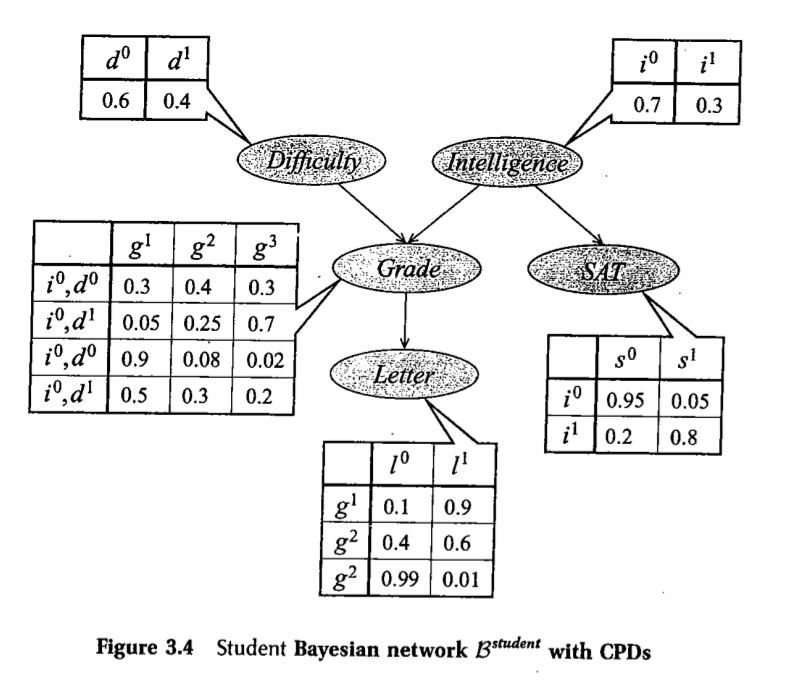
\includegraphics[width=\textwidth]{media/examplebayesnet.png}

\subsection{Adapting the model}
We note that the above Bayesian model represents explicit factorization of
joint probability distribution of all the random variables.
\begin{align}
  P(I, D, G, S, L) &= P_I(I)P_D(D)P_{G|I,D}(G|I, D)P_{S|I}(S|I)P_{L|G}(L|G)
\end{align}
where each factor corresponds to a function that is defined in Figure 3.4.

Note that each function depends only on a subset of random variables, for
example, $P_I(.)$ only depends on $I$, and $P_{G|I,D}(.)$ depends only on
$G$,$I$ and $D$.

Such a factorization can be represented as something called a \emph{factor
graph} (Fig~\ref{fig:fg2}). 

\begin{figure}
  \centering
  \includegraphics[height=0.58\textwidth, trim=0 0in 0 0, clip]{media/bayes2factorgraph.pdf}
  %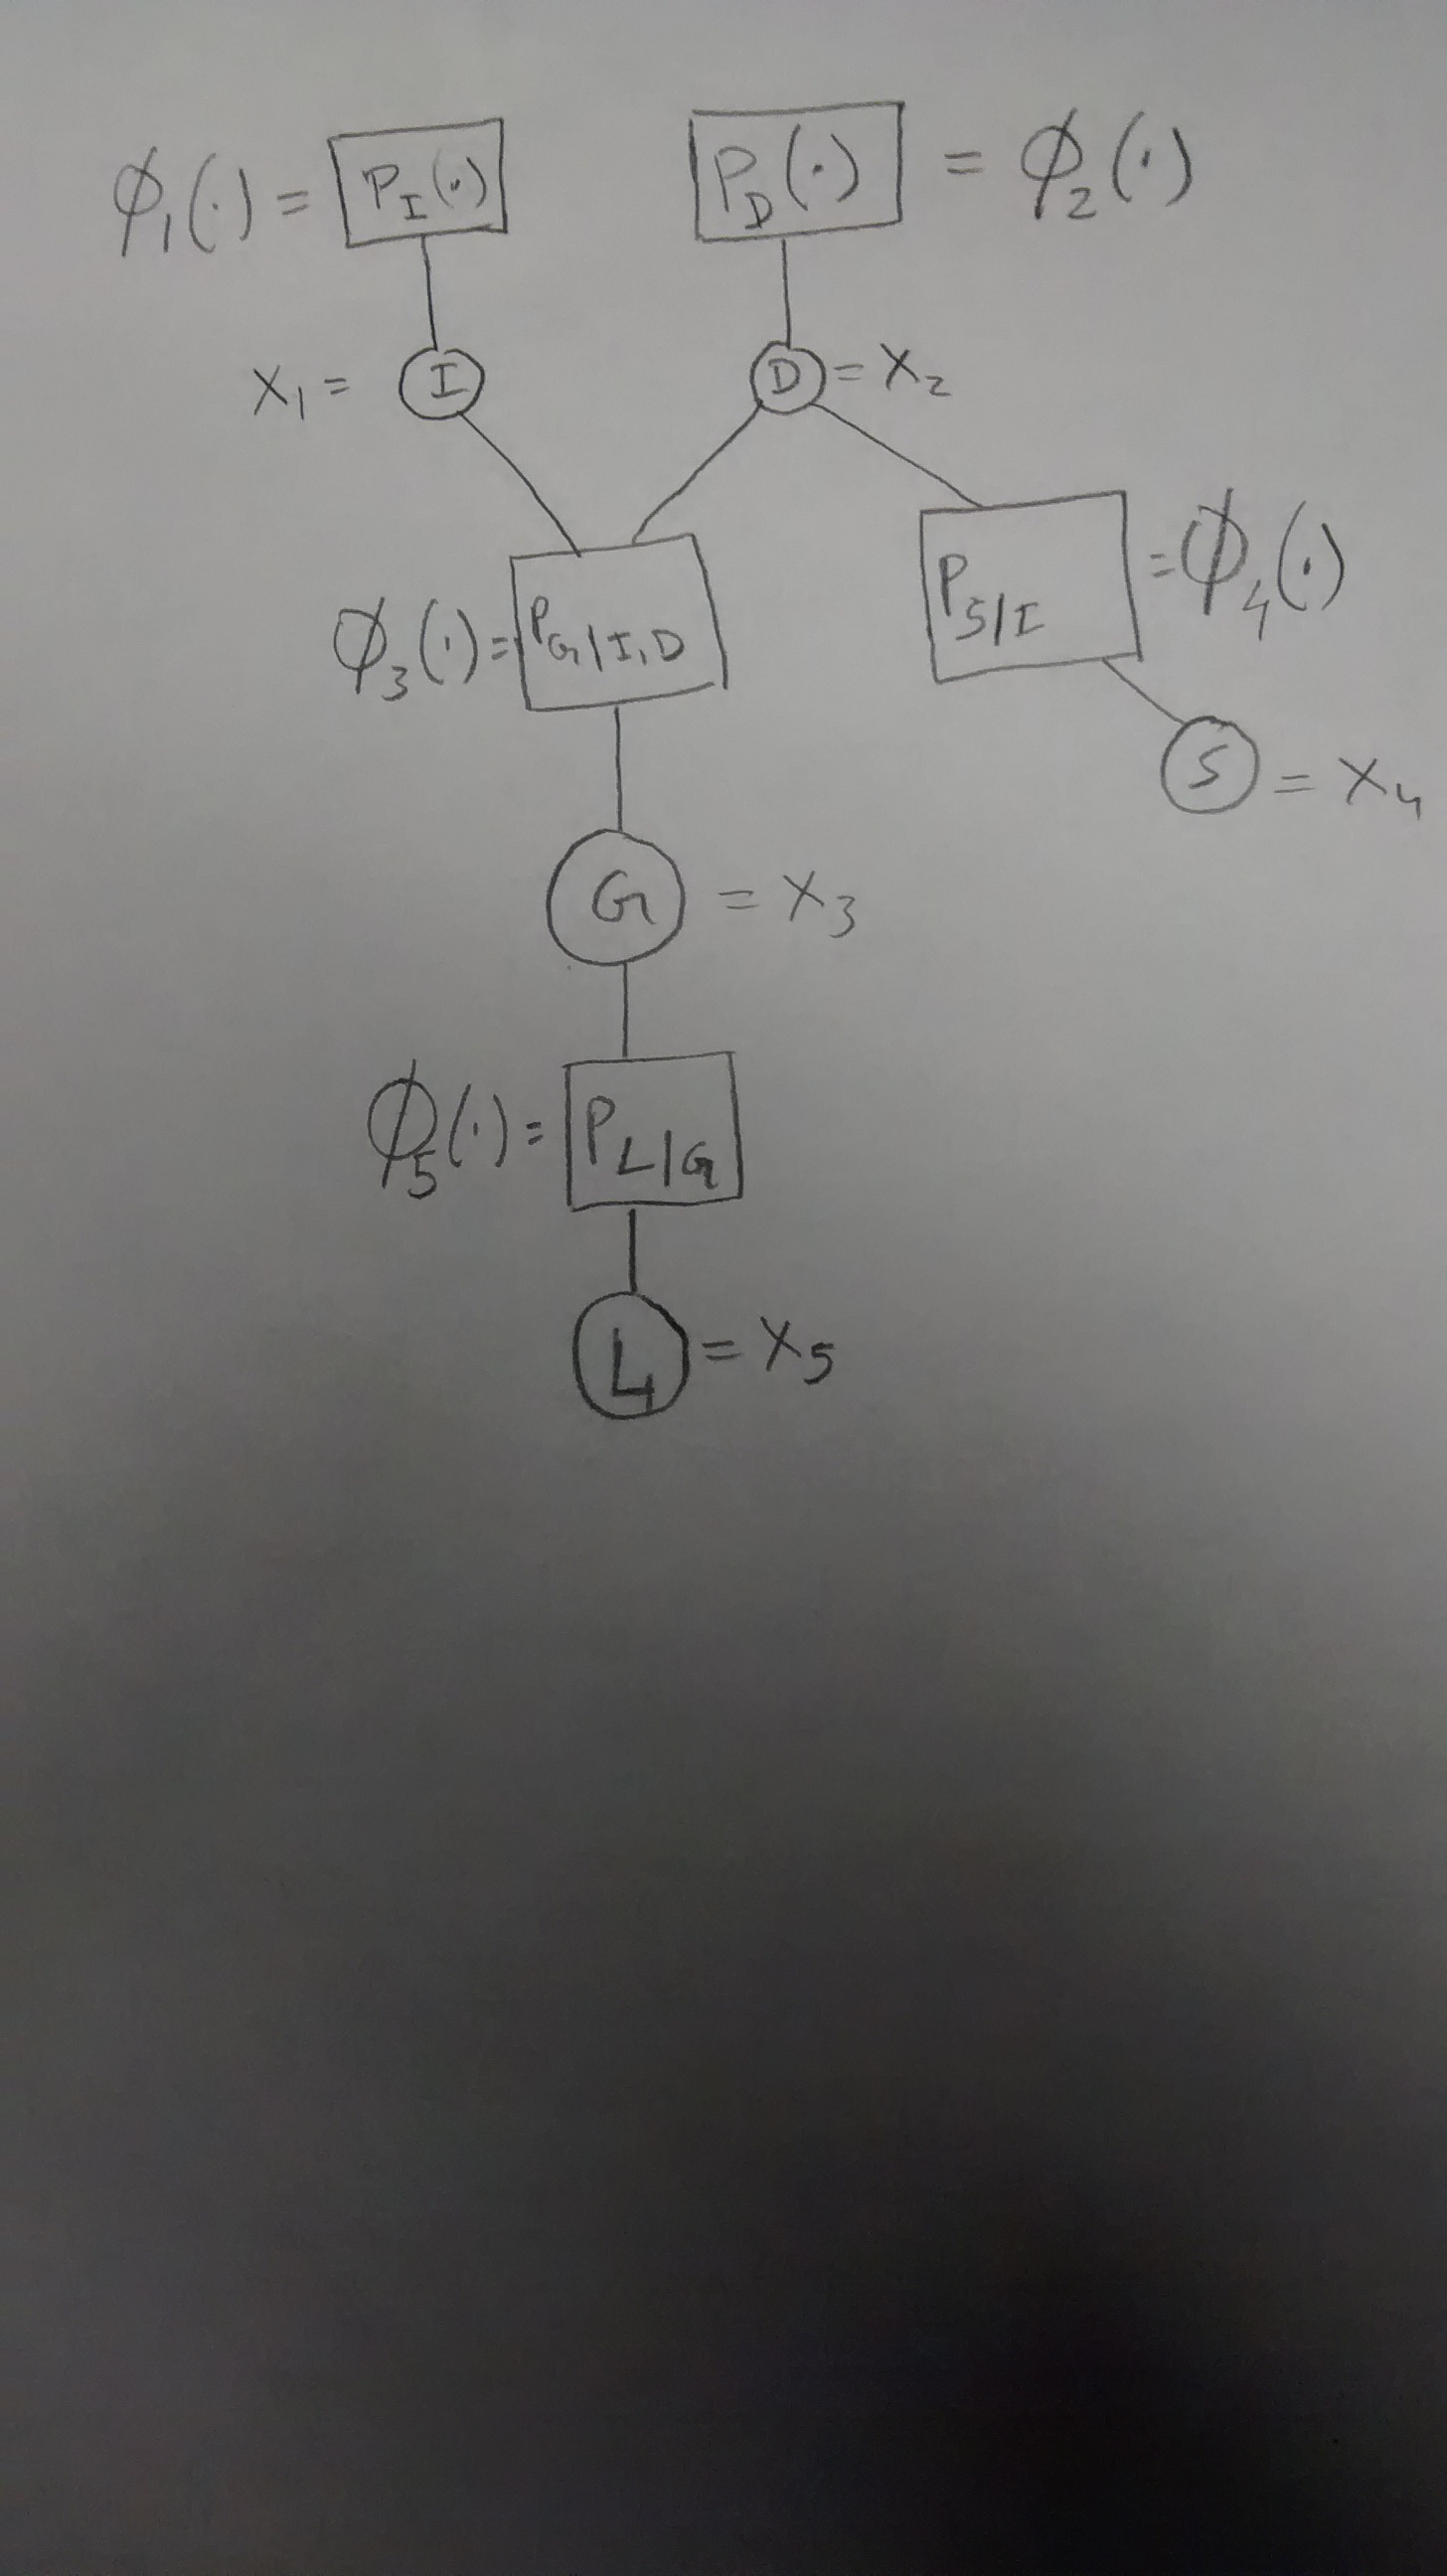
\includegraphics[height=0.58\textwidth, trim=0 15in 0 0, clip]{media/fg2.jpg}
  \caption{Factor graph representation}
  \label{fig:fg2}
\end{figure}

\subsection{Coding the graphical model}

For easier correspondence to the programmable graphical model we re-write our 
factorization in more general terms with the renaming of functions given in Table \ref{tab:rename}.
\begin{table}
  \centering
  \begin{tabular}{|l|l|}
    \hline
    Old factor name & New name \\
    \hline
          $P_D(.)$  & $\phi_0(.)$\\
          $P_I(.)$  & $\phi_1(.)$\\
    $P_{G|I,D}(.)$  & $\phi_2(.)$\\
      $P_{S|I}(.)$  & $\phi_3(.)$\\
      $P_{L|G}(.)$  & $\phi_4(.)$\\
    \hline
  \end{tabular}
  \begin{tabular}{|l|l|}
    \hline
    Old variable name & New name \\
    \hline
                  $D$ & $X_0$\\
                  $I$ & $X_1$\\
                  $G$ & $X_2$\\
                  $S$ & $X_3$\\
                  $L$ & $X_4$ \\
    \hline
  \end{tabular}
  \caption{Renaming factors to a more generic form}
  \label{tab:rename}
\end{table}

\begin{align}
  P(I, D, G, S, L) &= \prod_{i=0}^{4} \phi_i(\{ x_j \}_{j : \phi_i(.) \text{ depends on } X_j})
  \label{eq:factorization}
\end{align}

At this point we want to initialize the templated
\lstinline|opengm::GraphicalModel| class from the library, which requires us to
identify ValueType, OperationType, FunctionType and SpaceType arguments. We
will build up the arguments one by one.

\begin{lstlisting}
  #include <opengm/graphicalmodel/graphicalmodel.hxx>
  typedef opengm::GraphicalModel<
          ValueType,
          OperationType,
          FunctionType,
          SpaceType
            > Model;
\end{lstlisting}

\subsubsection{Identifying the ValueType and OperationType}

While defining the graphical model, we have to first define the types of its
components. For this we note that all our factors $\phi_i(.)$ are of the form
$\phi_i : \{L_j\}_{j=1}^{k} \rightarrow \mathbb{R}$. It should be noted that
for a consistent graphical model, the codomain of all factors $\phi_i$ should
be consistent for valid graphical model. This codomain of all the factors is called
the \emph{ValueType}. Corresponding to the $\mathbb{R}$, we can use the CPP
datatypes like \lstinline|float| or \lstinline|double|.

Also note the operator between different factors in equation
\eqref{eq:factorization}, is multiplication. This operator acts upon the
codomain of factors $\phi_i$. The corresponding datatype in opengm is
\lstinline|opengm::Multiplier|.  Although factorization in typical usage is
always with respect to multiplication, but in abstract mathematics you can
always replace one operator with another as long as it satisfies certain
axioms. Here, the operator is required to satisfy the axioms of a commutative
monoid.

\begin{definition}
  A tuple $(S, \otimes, 1)$ is called commutative monoid if set $S$, binary operation $\otimes$ and identity element $1 \in S$ satisfy following axioms
  \begin{enumerate}
    \item Closure: $\forall a, b \in S, a \otimes b \in S$
    \item Associativity: $(a \otimes b) \otimes  c = a \otimes (b \otimes  c)$
    \item Identity: $\exists 1 \in S | \forall s \in S, s \otimes 1 = s$
    \item Commutativity: $a\otimes b = b\otimes a$
  \end{enumerate}
\end{definition}

We do not need the general definition of commutative monoid, as long as we know
that addition and multiplication operator satisfy these axioms on real numbers.
At this point we can define the following properties of factor graph to be
representable in OpenGM

\begin{definition}
A \emph{factor graph} representation of a factorization 
$\phi(V) = \otimes_{j=1}^M \phi_j(v \subseteq V)$ 
is a three-tuple $(V, F, E)$ where 
\begin{enumerate}
   \item $V = \{X_i\}_{i=1}^{N}$ is a set of random variables 
   \item $F = \{\phi_j\}_{j=1}^{M}$ is a set of functions (or factors)
   \item $E = \{(X_i, \phi_j) | X_i \in V, \phi_j \in F, \phi_j(.) \text{ depends on } X_i\}$ is a set of underirected edges
   \item Each factor $\phi_j : L_j \rightarrow S$ has codomain in $S$.
   \item $S$ forms a commutative monoid with operator $\otimes$.
\end{enumerate}
\end{definition}

Programmatically, the \emph{ValueType} is corresponds to $S$. the
\emph{OperatorType} corresponds to $\otimes$.  In our example, $S$ is set of real numbers, hence ValueType is float or double;
$\otimes$ is simple multiplication, and OperationType corresponds to
\lstinline|opengm::Multiplier|.

% Note that data types/classes like \lstinline|opengm::Multiplier| and
% \lstinline|opengm::Adder| corresponds to the complete monoid instead of the
% operator of the monoid.

The ability of using addition operator (\lstinline|opengm::Adder|) in place
of multiplication is of practical importance, as it enables the use of log
domain for computation without modifying the graphical model. Log domain avoids
numerical problems like underflow that are common in probablistic graphical models.


\begin{align}
  \log P(I, D, G, S, L) &= \sum_{i=0}^{4} \log( \phi_i(\{ x_j \}_{j : \phi_i(.) \text{ depends on } X_j}) )
  \label{eq:factorization}
\end{align}

\subsubsection{Representing the factors} 

Next step is choosing the data type for representation of factors $\phi_i(.)$.
If the corresponding function can be tabulated, then the factor can be
represented as \lstinline|opengm::ExplicitFunction|. Depending upon the structure of 
factors $\phi_i(.)$ different classes can be used. The available classes of
functions is tabulated in Table 2.1 of the manual.

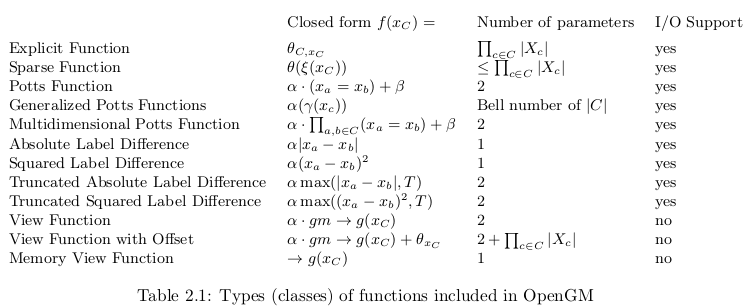
\includegraphics[width=\textwidth, trim=0 0 0 0, clip]{media/availablefunctions.png}

\begin{align}
  P_{G|I,D}(g, i, d) &= P_{G|I,D}(x_2, x_0, x_1) \\
                     &= \phi_2(x_2, x_0, x_1)
\end{align}

From the table of figure 3.4 we can explicitly assign the values for $\phi_2$

\begin{lstlisting}
  #include <opengm/functions/explicit_function.hxx>

  // Size of value space of each random variable i.e. X0, X1, X2
  size_t shape2[] = {2, 2, 3};
  opengm::ExplicitFunction<double> phi2(shape2, shape2 + 3, 0.0);
  phi2(0, 0, 0) = 0.3;  phi2(0, 0, 1) = 0.4;  phi2(0, 0, 2) = 0.3;
  phi2(1, 0, 0) = 0.05; phi2(1, 0, 1) = 0.25; phi2(1, 0, 2) = 0.7;
  phi2(0, 1, 0) = 0.9;  phi2(0, 1, 1) = 0.08; phi2(0, 1, 2) = 0.02;
  phi2(1, 1, 0) = 0.5;  phi2(1, 1, 1) = 0.3;  phi2(1, 1, 2) = 0.2;
\end{lstlisting}


\subsubsection{Representing the variables}

In this course we will be dealing with discrete spaces. The general datatype to
define discrete spaces is \lstinline|opengm::DiscreteSpace|. To define and
understand this we need to tabulate the variables involved in the graphical
model and their value (or label) spaces.

\begin{tabular}{|l|l|l|r|}
  \hline
  Random Variable & Original notation & Value space & Size of Value space \\
  \hline
  $X_0$ & D & $\{d^0, d^1\}$ & 2\\
  $X_1$ & I & $\{i^0, i^1\}$ & 2\\
  $X_2$ & G & $\{g^0, g^1, g^2\}$ & 3\\
  $X_3$ & S & $\{s^0, s^1\}$ & 2\\
  $X_4$ & L & $\{l^0, l^1\}$ & 2\\
  \hline
\end{tabular}

Our representation does not requires or allows special value spaces like
$\{d^0, d^1\}$ or $\{i^0, i^1\}$ for different random variables. 
Instead all discrete value spaces are completely defined by the size of label
space. If the size of label space is $L$, then the random variable can take
values from $\{0, 1, \dots, L - 1\}$.

Hence a discrete space can be simply be defined as 

\begin{lstlisting}
  #include <opengm/graphicalmodel/space/discretespace.hxx>

  opengm::DiscreteSpace<> space;
  space.addVariable(2); // X0
  space.addVariable(2); // X1
  space.addVariable(3); // X2
  space.addVariable(2); // X3
  space.addVariable(2); // X4
\end{lstlisting}

\subsubsection{Composing the graph}

Once we have initialized the factors and variables, we need connect the factors
and variables to complete the graph. At this point we should note a
difference in terminology. OpenGM distinguishes between a Factor and a
function.  The distinction arises when we can reuse certain functions. For
example, if we had $P_{L|G}(\mathbf{x}) = P_{S|I}(\mathbf{x}) \forall
\mathbf{x}$, then we could have represented both the factors with a same
function.

\begin{lstlisting}
  GMType gm(space);
  typedef GMType::FunctionIndentifier GMFunctionIndentifier;
  GMFunctionIndentifier fid0 = gm.addFunction(phi0);
  GMFunctionIndentifier fid1 = gm.addFunction(phi1);
  GMFunctionIndentifier fid2 = gm.addFunction(phi2);
  GMFunctionIndentifier fid3 = gm.addFunction(phi3);
  GMFunctionIndentifier fid4 = gm.addFunction(phi4);

  gm.addFactor(fid0, var0, var0 + 1);
  gm.addFactor(fid1, var1, var1 + 1);
  gm.addFactor(fid2, var2, var2 + 3);
  gm.addFactor(fid3, var3, var3 + 2);
  gm.addFactor(fid4, var4, var4 + 2);
\end{lstlisting}


\subsection{Queries}
Suppose we want to find out the probability of Letter being $l^1$.
Mathematically we want to find

\begin{align}
  P(L = l^1) = \sum_{D,I,G,S,L=l^1} P(I, D, G, S, L)
  \label{eq:marginal}
\end{align}

A similar but different that occurs often in PGMs is that of finding the Letter
that maximizes the joint probability. This is not exactly, the MAP query but
similar. Since OpenGM does not distinguishes between posterior or joint
probability, the difference needs to be handled during the factor graph
formulation. This method illustrates how you will be setting up inference for
MAP queries. 

\begin{align}
  L^* = \arg \max_{L} P(I, D, G, S, L)
  \label{eq:map}
\end{align}

This problem is called computing the marginal with respect to $L = l^1$. Not
all inference algorithms support computation of marginals. Belief propagation
is a kind of message passing algorithm that does supporting computing of
marginals. We will initialize Belief Propgation algorithm and compute the
marginals with following code. The template for setting up of inference
algorithms, is provided in the OpenGM manual. 

\begin{lstlisting}
  // Set up inference method
  typedef opengm::BeliefPropagationUpdateRules<Model, opengm::Integrator>
    UpdateRules;
  typedef opengm::MessagePassing<Model, opengm::Integrator, UpdateRules,
          opengm::MaxDistance> BeliefPropagation;
\end{lstlisting}

Note the use of \lstinline|opengm::Integrator|. It is because of the summation,
operator in the marginal problem \eqref{eq:marginal}. If we want to
solve for the MAP problem \eqref{eq:map}, we use \lstinline|opengm::Maximizer| 
instead of \lstinline|opengm::Integrator|. The rest of the code for setting up parameters and running inference is standard.

\begin{lstlisting}
  const size_t maxNumberOfIterations = 100;
  const double convergenceBound = 1e-7;
  const double damping = 0.0;
  BeliefPropagation::Parameter parameter(maxNumberOfIterations,
      convergenceBound, damping);
  parameter.useNormalization_ = true;

  // Inference on graphical model
  BeliefPropagation bp(gm, parameter);
  bp.infer();

\end{lstlisting}

While accessing the results, we can either ask for optimal labelings or marginal probabilities or both.

\begin{lstlisting}

  // Accessing marginal probabilities
  Model::IndependentFactorType marg;
  for(IndexType var=0; var<gm.numberOfVariables(); ++var)
  {
    std::cout<< "Variable x_" << var 
      << " has the following marginal distribution P(x_"<<var<<") :";
    bp.marginal(var,marg);
    for(LabelType i=0; i<gm.numberOfLabels(var); ++i)
      std::cout <<marg(&i) << " ";
    std::cout<<std::endl;
  }   

  // Find most likely labeling
  std::vector<size_t> labeling(gm.numberOfVariables());
  bp.arg(labeling);
  std::cout << "Labeling : " << ;
  for(IndexType var=0; var<gm.numberOfVariables(); ++var)
    std::cout << labeling[var] << ", ";
\end{lstlisting}

\section{Unresolved doubts}
There are a few things about the library that I don't understand. I have
written to the author for clarification, and hope to find out an answer soon.

\begin{enumerate}
  \item IndependentFactorType and Factor arithmetic: Why is it important and what kind of problems can factor arithmetic solve?
  \item How to compute marginal over multiple variables?
\end{enumerate}


\end{document}
